
\chapter{Exercise 1}

\section{Question 1}

\subsection{Compute the expectation and the variance of this distribution}
\subsubsection{Expectation}

\begin{align}
    \begin{split}
        P(X=k) =& \; \frac{\lambda^k e^{-\lambda}}{k!} \;\; ; \; X \sim P(\lambda) \\
        E[X] =& \; \sum_{k=0}^{\infty} k \cdot P(X=k) \\
        \Rightarrow \; E[X] =& \; \sum_{k=0}^{\infty} k \cdot \frac{\lambda^k \cdot e^{-\lambda}}{k!} \\
        \Rightarrow \; E[X] =& \; \sum_{k=1}^{\infty} \frac{\lambda^{k} e^{-\lambda}}{(k-1)!} \\
        \Rightarrow \; E[X] =& \; \lambda e^{-\lambda} \cdot \sum_{k=1}^{\infty} \frac{\lambda^{k-1}}{(k-1)!} \;\; ; \;\; \lim_{n \to \infty} \sum_{n}^{\infty} \frac{\lambda^n}{n!} = e^{\lambda} \\
        \Rightarrow \; E[X] =& \; \lambda e^{-\lambda} e^{\lambda} \\
        \Rightarrow \; E[X] =& \; \lambda
    \end{split}
\end{align}

As we can see, the estimator is the mean of the sample. The expected value of a Poisson random variable is equal to its paramenter $\lambda$, therefore the sample mean is an unbiased estimator of the expected value.

\subsubsection{Variance}

\begin{align}
    \begin{split}
        P(X=k) =& \; \frac{\lambda^k e^{-\lambda}}{k!} \;\; ; \; X \sim P(\lambda) \\
        Var[X] =& \; E[X^2] - E^2[X] \\
        \Rightarrow \; Var[X] =& \; \sum_{k=0}^{\infty} k^2 \cdot P(X=k) \; - \lambda^2 \\ \\
        E[X^2] =& \sum_{k=0}^{\infty} k^2 \cdot \frac{\lambda^k \cdot e^{-\lambda}}{k!} \\
        \Rightarrow \; E[X^2] =& \; \lambda e^{-\lambda} \cdot \sum_{k=1}^{\infty} k \cdot \frac{\lambda^{k-1}}{(k-1)!} \\
        \Rightarrow \; E[X^2] =& \; \lambda e^{-\lambda} \cdot \left( \sum_{k=1}^{\infty} (k-1) \frac{\lambda^{k-1}}{(k-1)!} + \sum_{k=1}^{\infty} \frac{\lambda^{k-1}}{(k-1)!} \right) \\
        \Rightarrow \; E[X^2] =& \; \lambda e^{-\lambda} \cdot \left( \lambda \cdot \sum_{k=1}^{\infty} \frac{\lambda^{k-2}}{(k-2)!} + \sum_{k=1}^{\infty} \frac{\lambda^{k-1}}{(k-1)!} \right) \;\; ; \;\; \lim_{n \to \infty} \sum_{n}^{\infty} \frac{\lambda^n}{n!} = e^{\lambda} \\
        \Rightarrow \; E[X^2] =& \; \lambda e^{-\lambda} \cdot (\lambda e^{\lambda} + e^{\lambda}) \\
        \Rightarrow \; E[X^2] =& \; \lambda^2 + \lambda \\ \\
        \Rightarrow \; Var[X] =& \; \lambda^2 + \lambda - \lambda^2 \\
        \Rightarrow \; Var[X] =& \; \lambda
    \end{split}
\end{align}

Again, the variance of a Poisson random variable is equal to its parameter $\lambda$.

\section{Question 2}
There are several reasons, first of all $\lambda$ is the only parameter we need to define the Poisson distribution, once $\lambda$ is known then mean and variance follow effortlessly as seen in the previous exercise.
The Poisson distribution also possess another interesting and useful property: the Markov property (memorylessness). In probabilistic forecasting is a desirable property that may enable a simplified way to the solution of complex problems.
The estimator $\lambda$ distributes exactly like a Poisson distribution with parameter n$\lambda$. This distribution, for a sufficient big n can be approximated by the Normal distribution with same average and variance as the relative Poisson distribution.

\section{Question 3}

Figure \ref{fig1} shows the distribution of the average of a sample drawn randomly from a Poisson distribution with $\lambda=0.5$. 
\begin{figure}[ht]
\centering
\includegraphics[width=10cm, angle=270]{Q1_3plot.eps}
\caption{Poisson distribution}
\label{fig1}
\end{figure}
We can make two observations. On the one hand, we can see that our estimator is unbiased, the distribution is centered on 0.5 and we clearly see the impact of the number of observations on the 4th momentum (Kurtosis). On the other hand, as the sample size grows, we have a more precise estimation, the estimation is more efficient, its variance decreases, resulting in a peak in the density plot.


\section{Question 4}
Figure \ref{fig2} shows the standard deviation of the Poisson distribution with  $\lambda=0.5$ and different sample sizes. It shows the the impact of the number of observations on the estimator's volatility. We observe that as the sample size grows, the volatility of the estimator decreases and its efficiency increases.  The marginal change in speed of convergence is descending and we can reach a reasonably good measure (i.e. converge to the real value) with relatively few observations.

\begin{figure}[H]
\centering
\includegraphics[width=10cm, angle=270]{Q1_4plot.eps}
\caption{Estimated volatility of the estimator (Poisson distribution with $\lambda=0.5$)}
\label{fig2}
\end{figure}


\section{Question 5}

Figure \ref{fig3}  demonstrates the central limit theorem. We compare the distribution of our sample mean drawn from a Poisson distribution to the normal distribution. More precisely we compare
\begin{equation*}
\frac{\sqrt{n}(\frac{\sum{x_i}}{n}-\lambda)}{\sqrt{\lambda}} \qquad \textrm{ with } \qquad N(0,1)
\end{equation*}
The central limit theorem states that as the sample size goes to $\infty$, the distribution of the sample mean, drawn from any distribution with finite moments, will asymptotically converge to the normal distribution.  We can clearly state that the convergence in distribution towards a Normal distribution is very quick and remains accurate even with a small number of observations. Again, the estimator itself is a random variable!

\begin{figure}[ht]
\centering
\includegraphics[width=10cm, angle=270]{Q1_5plot.eps}
\caption{Demonstration of the Central Limit Theorem}
\label{fig3}
\end{figure}

